\documentclass{article}
\usepackage[utf8]{inputenc}
\usepackage{graphicx}

\title{Assignment 0}
\author{Frederik Rothe}
\date{September 2021}

\begin{document}

\maketitle

\section{IsLeapYear()}

The IsLeapYear() method contains a very simple algorithm determining whether the year that the user inputs is a leap year. 
This is done with the use of two if-statements. \\
Firstly, we check if the number is divisible by four, if not we discard it right away and return false. However, if the number is in fact divisible by four we have a candidate for a leap year. \\
Hereafter, we have the second if-statement to determine if that candidate really is a leap year. The rules of leap years say that years divisible by 100 is not a leap year, except \textbf{iff} the number is divisible by 400, then it is in fact a leap year. \\
This concludes our algorithm.

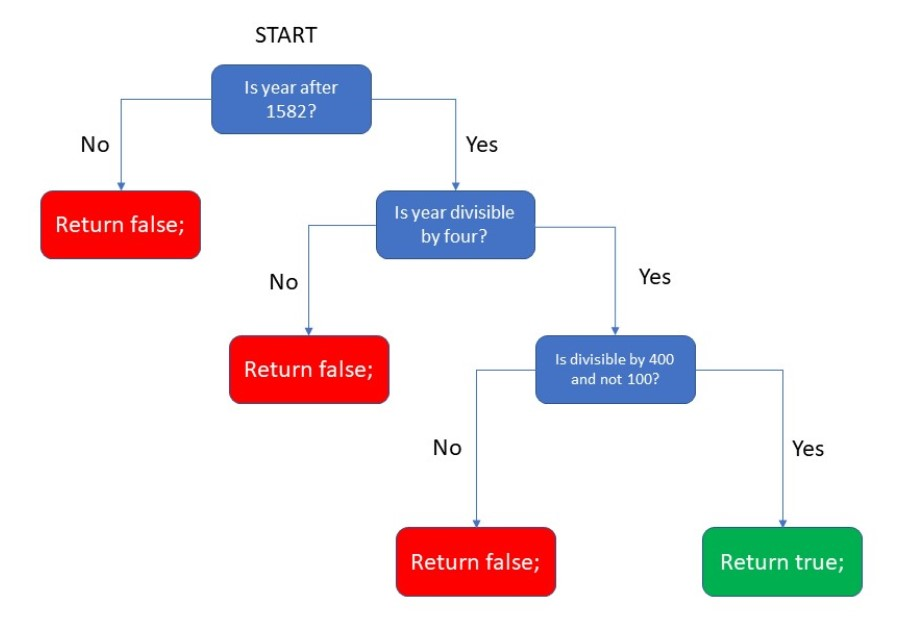
\includegraphics[width=350p,height=200p]{IsLeapYearDiagram.jpg}

\end{document}
